\documentclass[14pt]{beamer}
\usetheme{Luebeck} %Malmoe
\setbeamertemplate{footline}[frame number]
\setbeamertemplate{navigation symbols}{}

\usepackage[english]{babel}
\usepackage[latin1]{inputenc}

\title{Methodology of Construction of GCC Front-End}

\author[Petr Machata]{Petr Machata \\ \texttt{xmacha31@stud.fit.vutbr.cz}}
\date{2007-20-06}

\begin{document}

\frame{\titlepage}

\frame
{
  \frametitle{About My Project}

  \begin{itemize}
  \item ``Methodology of Construction of Compiler Front-End and Its
    Integration into the GNU Compiler Collection''
    \begin{itemize}
    \item Or: ``Howto support prog. language via GCC''
    \end{itemize}
  \end{itemize}

  \begin{itemize}
  \item The side effect: Algol 60 compiler
  \item Personal ambition: widely accessible
    \begin{itemize}
    \item English, Open Source
    \end{itemize}
  \end{itemize}
}

\frame
{
  \frametitle{Language Support in General}

  \begin{itemize}
  \item Language support:
    \begin{itemize}
    \item Compilation
    \item Runtime support
    \item Debugging support
    \item C binding
    \end{itemize}
  \end{itemize}
}

\frame
{
  \frametitle{GCC Architecture}

  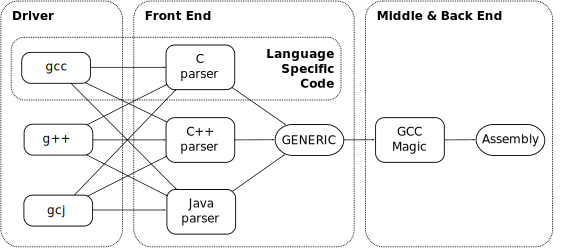
\includegraphics[height=4.8cm]{demo-gccarch.pdf}
}

\frame
{
  \frametitle{Language Support via GCC}

  \begin{itemize}
  \item Why GCC
    \begin{itemize}
    \item Vast community: users, OS vendors, researchers
    \item C on steroids
    \item Sophisticated optimizations
    \item Debuginfo almost for free, near 1:1 accurate
    \end{itemize}

  \item GCC goodies
    \begin{itemize}
    \item Automatic preprocessing
    \item Automatic linking
    \item OpenMP support
    \item Inline assembly
    \item Builtins (lots: ISO C, threads, whole glibc!)
    \end{itemize}
  \end{itemize}
}

\frame
{
  \frametitle{Summay of a Work}

  \begin{itemize}
  \item {\tt gcc-algol} can compile most of Algol 60
    \begin{itemize}
    \item No functions (Algol functions are hard)
    \item Runtime library: \texttt{puts}, \texttt{exit}, \texttt{**}
    \item Uses C preprocessor
    \item Emits debuginfo
    \end{itemize}
  \end{itemize}
}


\frame
{
  \frametitle{Questions?}

  \begin{itemize}
  \item Questions?
  \end{itemize}
}

\end{document}

% Local Variables:
% compile-command: "make show-demo-2"
% End:
